\documentclass[journal]{IEEEtran}
\usepackage{graphicx}
\begin{document}

\title{Operating System Multi-Core Scalability Issues}

\author{Edward~Hills}

% make the title area
\maketitle

\begin{abstract}

Multi-core scalability is in the fore-front of every programmers mind when programming operating systems or any serious modern applications. For a number of years now it has been impossible to increase a single cores clock speed due to several limitations, mainly heat and power consumption. This is why a new paradigm has arisen in which we put more and more cores into a single CPU. Due to Moore's Law we know that the number of transistors that we can fit onto a single chip doubles roughly every 18 months. With this the next decade is expected to herald 100s or even 1000s of cores on a single chip. This is why we must begin to start thinking about how we can scale our operating systems and applications to gain the full benefit of the massively multi-core paradigm. This paper will talk about some current and future methods to attack scalability, as well as propose some new ideas.

\end{abstract}

\section{Introduction}
\IEEEPARstart{S}{calability} is an important issue in todays modern operating system era. Current operating systems (OSs) are being retro-fitted with techniques to increase their scalability. On a whole things are improving, and this can be seen in the latest versions of the Linux kernel which are being released. However, some researchers see this is a stop-gap rather than a solution. This is due to a number of factors which cannot simply be `patched' to be more scalable due to their semantics. Some scalability issues include:

\vspace{2mm}

\begin{itemize}
\item Global or coarse-grained locks,
\item TLBs,
\item Shared Memory,
\item Semantic Serialization,
\item Cache misses, and
\item Unnecessary Resource Sharing
\end{itemize}

\vspace{5mm}

Coarse-grained locks are a major scalability issue in multi-core and highly threaded systems. A coarse-grained lock locks a larger area than it needs to accomplish a job that needs to be run without interference or the possibility of a race condition. Original Linux kernels have had whole kernel global locks as these were the easiest for the developers to implement, however these were quickly removed with smaller and finer-grained locks as multi-core became more apparent. Unfortunately these locks are still not fine-grained enough in todays increasingly multi-core environment.

TLBs or Translation Look-aside Buffers, holds a table of physical addresses which have been mapped from virtual addresses, these are generally needed to be global so that each core gets the same data. When updating or viewing the TLB a lock must be held which stops all other processes from accessing it to avoid race-conditions and unwanted side effects. TLBs are a widely used data structure which in its generic form can severely limit scalability.

Shared Memory is simply a region of memory that is shared amongst different cores (in our context), these can cause a range of scalability problems which are discussed later.

Semantic serialization is the problem in which some code blocks must be run in serial due to the nature of their task. These are some of the hardest problems to overcome as the semantics need to be rethought and designed completely to be able to semantically remove these.

Having one core read what another core just wrote imposes a wide range of cache misses. If the same core that did the writing did the reading then it would be able to access the data from cache (about 10-50 cycles) and save it from accessing memory (about 100-300 cycles).

Unnecessary resource sharing often occurs as side effects of bad programming or lack of thinking about scalability. Some resources simply do not need to be shared and we will see examples of this later.

Throwing more cores or processors at a problem may not be the ultimate solution however, as Amdahls Law \cite{Amdahl} shows. We are instead limited by the sections which must be run in serial, if a program spends 1 hour out of 20 (95\%) executing serial code then Amdahls Law states that we can only speed up computation by 20x no matter how many cores we have. This is why serial parts of a system must be carefully rethought and redesigned to be parallelized. \emph{Fig. \ref{AmdahlGraph}} shows Amdahls findings. 

\begin{figure}
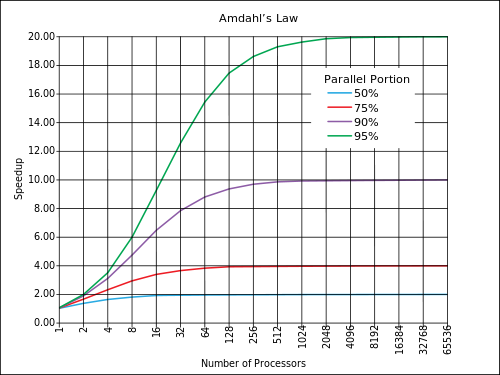
\includegraphics[width =9cm, height =8cm]{Amdahl.png}
\caption{Amdahls Findings. Sourced from Wikipedia.}
\label{AmdahlGraph}
\end{figure}

In this paper I will talk about previous papers and the techniques which have helped overcome these problems such as \emph{sloppy counters} \cite{sloppy-counters}, \emph{Read-Copy-Update} techniques \cite{RCU} and OSs which have done a full re-think of the kernel design with scalability in mind such as \emph{fos} \cite{fos}.

After briefly talking about the different paradigms for tackling OS scalability I will then talk about a new idea which I propose will help increase scalability in a future massively multi-core operating system. My idea follows on from the general design and idea of fos which I will describe soon. My idea is to basically associate each core with a device or resource which can help reduce contention for that device as only one core will be interacting with the device and will implicitly take out a global lock on that device.

\section{Related Work}

Multi-core CPUs have been around for over a decade now and have had plenty of time to adjust and come up with new ideas to help improve the scalability issues that we face. This section will discuss some issues and previous solutions to overcome these, as well as some new designs and ways of thinking about the issue of scalability. 

\subsection{Current OS Solutions}

Without changing drastically the way we think about modern operating systems we have no choice but to examine areas of the kernel we have now and find ways to limit the amount, what, where and when we share resources among each thread or core. By reducing the amount of sharing we have to do and by keeping everything as modular as we can, we can try and curb the amount of differing cores that must access the same object. By doing this, we can improve scalability drastically. 

\subsubsection{Sloppy Counters}
\emph{Sloppy counters} proposed by Boyd-Wickizer \emph{et al.} is a way of doing \emph{lazy updates}. The Linux kernel uses shared counters for a range of tasks such as managing resources and garbage collection, this is a scalability issue if many cores are accessing and updating these counters. \emph{Sloppy counters} aims to remove this bottleneck by having each core have its own counter and update its per-core counter instead of the shared counter. It does this in the hopes that it can keep spare references that new threads can use. It will have to reconcile with the central counter if the local count grows above a certain threshold value or when deciding whether an object should be deallocated, thus it is best used when objects are rarely deallocated.  

Sloppy counters has the added benefit of being backwards compatible with other kernel counters meaning that not all sections of the kernel need to be changed but only those which impose scalability issues. However one down side is that that they use space proportional to the total number of cores.

By adding sloppy counters to keep track of \emph{dentrys}, \emph{vfsmounts}, \emph{dst\_entrys} (which are very frequently used in applications such as Apache) and to keep track of memory allocated by TCP and UDP network protocols we can vastly improve scalability in the kernel. In fact, Boyd-Wickizer \emph{et al.} found that by doing the above and one or two other improvements, the scalability of Apache was increased by several orders of magnitude. \cite{sloppy-counters}

One downfall of this paper \cite{sloppy-counters} is that it does not give specific quantifiable results when using just sloppy counters, this is because the paper benchmarks a range of applications with more than one improvement made to it which is unfortunate considering their new method to improve scalability was sloppy counters.

\subsubsection{Read-Copy-Update}
Read-Copy-Update provides a solution to many scalability issues, an important one being contention in the address space design \cite{Bonsai}. Clements \emph{et al.} re-designed the address space to use a balanced binary tree, \emph{Bonsai}, to ensure non-destructive updates of the table.

I will now briefly describe RCU and how it helps with scalability in a multi-core environment.

The main idea of RCU is that when a reader process or thread comes to read a particular block that is inside an RCU synchronization block, it first copies the data that is held within the data structure and then makes a copy of the original pointer itself. Next, it simply carries on and if need be it updates its copy. It then updates the global pointer and waits a certain grace period. It has this grace period so that all other readers which are reading the original data structure have time to finish before the update is complete. 

Once the code enters a `quiescent state' (an area in the code in which you can guarantee that all previous operations have completed) then the grace period ends and the resource is reclaimed. There are several things that defines what a `quiescent state' is, some methods simply use a counter and increment every time an operation is begun and decrement it when an operation is finished, then when the counter reaches zero it has completed everything before it. For non-preemptive systems, if a context switch is performed then that could be classed as a quiescent state also. In some systems if an interrupt is called or a trap has been executed then these are also accepted.

RCU in its standard implementation is mainly used for read-mostly data structures such as a routing table which is more often read than updated. One major advantage to RCU is its low-cost and low-overhead compared to normal synchronization techniques (such as a spinlock) which is relatively expensive and multi-processor unfriendly.

RCU is described as a `two-phase' locking mechanism, the first phase is to carry out enough of each update for new operations to see the new state, but still let old operations carry on. The second phase is to finish the update once the grace period has finished.

RCU has a severe advantage over traditional locking mechanisms such as spinlocks as they are severely limited by worst-case memory latency. This is because once a traditional lock has been obtained it must write to the locked data-structure, this means that it must hit memory which is slow compared to cpu or cache.

There is however a limitationdue to the \emph{wait\_for\_rcu()} function which does not work in a preemptible kernel unless preemption is specifically disabled for that section.

When implementing FD management with the use of RCU, Mckenney \emph{et al.} \cite{RCU} found that the kernel exhibited over 30\% more throughput for 4 cores and even with a uniprocessor there was a \emph{slight} increase in performance (0.65\%).

Multi-core oriented OSs such as K42 \cite{K42} use RCU pervasively as an existence lock. It has been in common use in Linux kernels since 2.5.

Read-Copy-Update locking technique allows multiple threads and cores to access the same data-structures without having to attain a lock which would limit scalability.

By applying RCU to a balanced binary tree \cite{Bonsai} \emph{Bonsai}, we are able to perform read operations in parallel with writes and avoid cache coherence traffic caused by read locks. \emph{Bonsai} avoids the race conditions of keeping the red-black tree balanced by its design.

By implementing \emph{Bonsai} into the Linux kernel, applications such as \emph{Metis} and \emph{Dedup} can achieve near-perfect increase in speedup to 80 cores and the results of Clements \emph{et al.} showed that the scalability improvement was likely to keep on being beneficial with even more cores.

\subsection{Future OS Solutions}

Techniques like the ones I have described above could be seen as `stop-gaps' to the scalability issues that we face in modern operating systems. These are becoming more and more effective as we devise new techniques for increasing scalability, however there are still some that believe a total rethink and redesign of operating systems needs to be done. Below I will talk about a couple of these.

\subsubsection{Factored Operating-System}

\emph{fos} or Factored Operating System \cite{fos}, is an operating system that has been designed with scalability at the forefront of the developers mind. Fos aims to be able to support future massively multi-core chips (1000+ cores) that are likely to be around in the next decade or so. It has done away with contemporary modern operating system design such as stock Linux and has instead been rethought and redesigned to work a lot like the Internet does today.

\begin{figure}
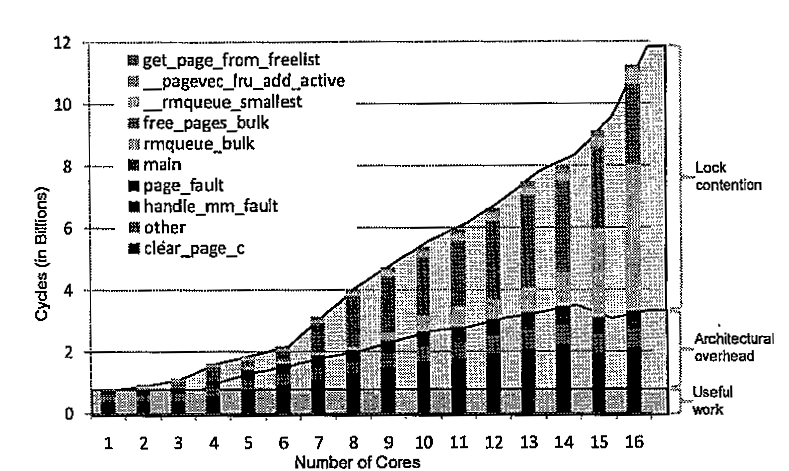
\includegraphics[width =9cm, height =8cm]{page_allocator.png}
\caption{Scalability of Physical Page Allocator. Sourced from \cite{fos}}
\label{PageAllocator}
\end{figure}

The image in \emph{Fig. \ref{PageAllocator}} shows an interesting result which \cite{fos} discovered. \emph{Fig. \ref{PageAllocator}} is a graph of the physical memory page allocator and its ability to scale. You can clearly see that the more cores that are added the less `useful' work is really done by the page allocator and the more time it spends waiting on locks. 

Fos takes its main fundamental idea from common Internet servers that are used everyday for the web. These servers are highly scalable and can deal with millions of users at a time. In a nutshell fos has a few separate and important ideas:

\vspace{2 mm}

\begin{enumerate}
\item Kernel and Application code execute on separate cores
\item Each core performs a set of separate services
\item Main communication between cores is via message passing
\item Sets of services and applications can be broken up into multiple \emph{fleets}
\item Traditional timesharing system is replaced with spatial sharing
\end{enumerate}

\vspace{5 mm}

By designing fos with the above view we instantly avoid the need for a majority of locks as well as avoided having the application and kernel interfere with each other. Below are just some of the benefits offered such as:

\vspace{2 mm}

\begin{itemize}
\item Inherently avoids contention between application and kernel
\item Only one thread for each core avoids locks
\item Quicker access to services and fully parallelized as tasks are spatially-shared not time-shared
\item Avoids expensive context switches
\end{itemize}

\vspace{5 mm}

The system service servers execute on top of a thin microkernel inspired by designs such as Mach \cite{Mach}, however there are a few differences such as distribution and parallelizing within a single system service server and having a spatially aware placement engine/scheduler. The lowest level of software management comes from the microkernel.

To describe further the relationship between fos and Internet Servers, fos even uses a cached namespace server (which provides fast lookup) and controls which messages get sent to which servers. This makes it possible for nodes to drop in and out (like the Internet) without losing important information because the name server will make sure it gets to where it needs to go and ensure at least one server takes the message. Messages are deposited into \emph{mailboxes}.

A typical server is designed to process a queue of requests, perform an action and send a reply. Servers are designed to be stateless, just like a lot of Internet services. This means that these are can be transaction-oriented and therefore requires no locking to stop threads updating memory. To further help scalability, servers acquire all resourced before the transaction starts and will only yield to the next transaction (fos is a non-preemptive system).

Due to fos being a message passing system there is no shared memory locks between cores so immediately a major scalability issue has been resolved. There is only ever one thread executing at a time on a server and there is no preemption therefore no locks are needed. To avoid sharing hardware structures such as caches and TLBs the OS servers operate on different to cores than that of applications. The final major advantage is that different parts of the system are also spatially separated so do not implicitly interfere with shared data structures.  

There are few issues with fos however and that is that it now has a large amount of core-to-core communication, however this cost is vastly less than that of shared memory (15-45 cycles compared to about 200 cycles respectively). Another issue is that replacing traditionally shared data structures such as the file systems buffer cache may not be possible and is currently unknown whether a hardware or software solution will be best. Another major question is if there are no locks being used within or between servers if a sequence of transactions can occur without some rare race conditions happening.

As you can see from my \emph{brief} discussion of fos above that it offers a new and \emph{less-is-more} approach to scalability. It takes a design which we see everyday in our lives, the Internet. The server-client model has been shown to allow massively scalable approaches and this is what fos aims to achieve also. By separating the services and applications spatially across a massively multi-core processor traditional operating techniques such as time-sharing is replaced. Fos is still in its developmental stage however but may be paving the way for future massively multi-core scalable operating systems.

\section{New Proposal}

In The previous sections I talked briefly about different ideas for obtaining good scalability in a multi-core system. The first way looked at attempting to change the way modern operating systems are trying to `patch' what they do now to allow further scalability such as using an RCU-friendly balanced binary tree for scalable address spaces. The second way I talked about was to completely rethink the design of operating systems and start from a new perspective where scalability comes first. 

My proposal to help scalability in operating systems carries on from fos which I have discussed above. I believe that fos is the way of the future in terms of scalability and simply `patching' modern OSs that we have today will eventually cease to provide benefits. This is why my question extends the ground work that fos has provided.

\subsection{Basic Idea}
My new idea to help improve scalability is to take a similar approach to that of \emph{fos} \cite{fos} and completely rethink the idea and design of the kernel. The client-server approach to operating systems that fos uses provides many benefits that I have discussed above. 

My proposal to further help scalability is to take the current idea of fos I have briefly explained above and add an extra layer of abstraction which will help avoid costly locks on common devices which often need to be shared such as the disk or RAM. On a 64+ core system, having 4-5 cores used up for device interfaces should not cost the much in overall performance to the main task of the system, especially with the future possibly bringing us 1000+ cores on a single chip in the near future. 

In fos, each core acts as its own server, it performs one tasks and sends and receives messages from other servers and applications, each operating on their own cores. However one issue which has not been resolved in fos is how locking common shared resources such as disk or RAM would be done. 

I propose that devoting an entire core (or possibly several cores) to a specific resource such as RAM or disk would help alleviate locking issues. The general idea would be that for each device there is a core tasked with interfacing with it. Each core that had something to be written or read from this device would first have to go through this \emph{interface core}. Having the one core which interfaces with say the disk, would allow that core to implicitly take out a global lock on the disk. This now explicitly makes the process of reading or writing something from disk explicitly asynchronous. 

For devices such as physical memory multiple cores could be given a range of addresses that it looks after and that way will shorten the queue of tasks to be written/read.

In the next section I will provide some further details as well as some examples to think about.

\subsection{Possible Implementation}

As talked about in the section above, my basic idea is to specify a core or set of cores which would be directly and solely tasked with interfacing with a particular device, RAM or the disk say. 

As talked about earlier fos uses a message passing system in a transaction like manner which contains all state that is required to complete a specific task. Having a message passing and mailbox system that fos has makes using my idea relatively easy.

The mailbox would act like a priority-queue (depending on the device if priority is important or not), which would contain a set of messages (or jobs) containing information to be read/written to the device. One could imagine a interface core for a disk which has two mailboxes (one for reading and one for writing) each containing many messages waiting to be written or read to disk, \emph{m$_{1}$, m$_{2}$, m$_{3}$ ... m$_{n}$}. The core would then process each message at a time (ignoring priorities for simplicity) and do what was required to the resource. If a new message \emph{m$_{n+1}$} was to come in, it would first check through the list of messages already waiting, check if what it wanted done interacted with a message already waiting (perhaps writing to the same line in a file say), it would then merge the two tasks if possible (a lot like source-control programs such as \emph{git} do) then combine the two messages into one. Given a large per-core cache these operations could be very quick saving on having to access shared memory which can be many orders of magnitude slower. You can this in \emph{Fig. \ref{MessageToDisk}.}

If a message which was to come along and want to read something from disk, it would first check the mailbox for writing to see if it was in the queue waiting to be written, if so it would simply grab that message and return that instead of accessing the disk.

\begin{figure}
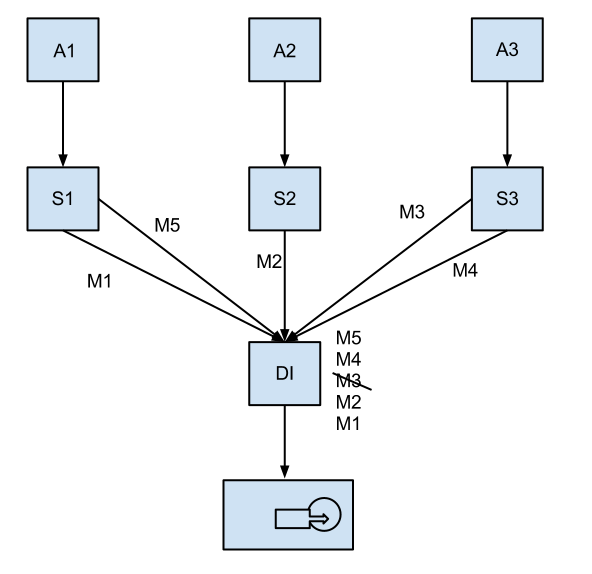
\includegraphics[height = 7.5cm, width=8.5cm]{MessagetoDisk.png}
\caption{Logical view of applications writing to the disk. A message is first passed from the application to a filesystem server and from there it's passed to the disk interface server. We can see that \emph{M4} arrives after \emph{M3} and \emph{M3} has been canceled due to \emph{M4} writing to the same position and therefore no longer needed. \emph{M1} is then processed by the disk and the response \emph{MR1} is propagated back to \emph{A1}.}
\label{MessageToDisk}
\end{figure}

The cost as previously mentioned for inter-core communication can be about 10-50 cycles, by adding these extra layers of indirection we are increasing the latency, however as has been said also this is still faster than the time it takes to access RAM. 

For devices such as RAM which can take up a large `space' and have large amounts of access we can dedicate one core to a range of addresses. We could say divide the full range of addresses and have one core for each quarter of the addresses. This is obviously an over simplification of how access to RAM works but the main principle still applies. Another point is that this would obviously be extremely slow as it is very simply and easily possible for an individual core to access and lock only the memory locations that it wishes to access, but the point still stands.

Having all these cores accessing different devices could severely limit the computational power of the system depending on how many cores there are in total. This is why I propose it should be possible for the cores which are acting as interfaces to be able to sleep and be used as other services or applications if not needed. The idea is that the core would relinquish (or at least suspend) control of the device and start executing something else. It would however stay in the name server so that when other cores wish to access the device they would still send messages its way and then that core would resume control of the device and carry on. Depending on the device, if it was to become inactive for a certain period of time, it could go to sleep (and start processing something useful). 

Due to fos and systems such as fos using a locality based approach, we are able to select cores which are in a position to provide the best performance for our needs. This way we are able to assign a core (or set of cores) which interfaces with, say the disk, so that we can afford the best performance, \emph{i.e.} have several of these cores arranged so that the distance each core has to send its message to is at a minimum. We can also assign cores which are closest to the I/O bus (if there is one) to avoid further distance. 

\subsubsection{Some Assumptions}
In the above I do make several assumptions which I will now state below.

The first assumption I make is that messages can be relatively quickly processed and that the queue would never grow to such a size that searching through it would be difficult or time consuming. This is generally the case with devices such as RAM which are not overly slow. For disk however, this may not prove possible. 

I also assume that the per-core cache is large enough to store the messages and that the mailbox will be large enough to accommodate the number of messages required.

I briefly mentioned that source-control systems such as Git use a merge algorithm to merge previous versions with newer versions, I am unsure of how this is accomplished but something similar could be used or modified to work with the needs stated above.

Another assumption is that the message passing system that fos describes can accommodate what needs to be done above, my current understanding is that it could. 

A fairly large assumption I make earlier is that the cores that are accessing the devices wont be missed. As fos looks to the future with 100+ or 1000+ cores, having half a dozen or so cores missing would be unlikely to be missed, even in a 64 core system, they are unlikely to be missed. I do try and address this problem above however by discussing the possibility of having them `sleep' from accessing the device and instead do some other work. This would however impose a cost when they wake up to process new information after `sleeping'.

\section{Conclusion}

In this paper I have discussed two competing ideas for improving scalability, `patching' modern operating system kernels and the much more drastic path, to completely rethink and redesign the kernel with scalability as the first concern. I then proposed my idea which is an extension of fos \cite{fos} and may help improve the issue of resource contention. I suggest that only allowing one core (or perhaps set of cores depending on the resource) to access a device. By doing this, that core implicitly takes out a global lock on the device and stops any contention issues. Due to the messaging system that fos uses it is relatively simple to make possible.

In the first section I talked about two techniques for improving scalability in current modern operating systems, \emph{sloppy counters} \cite{sloppy-counters} and \emph{Read-Copy-Update structures} \cite{RCU}. Both these have been widely used (RCU especially) to increase scalability in the kernel. Sloppy counters are a form of \emph{lazy counting} or \emph{distributed counters} which avoids needless communication and global counters needing locks. By replacing some explicit global counters with sloppy counters, vast improvement can be made as we avoid having to gain and lose multiple locks. RCU-friendly structures such as the \emph{Bonsai} tree can be used to have scalable concurrent address spaces and vastly improve scalability in the kernel \cite{Bonsai}.

In the second section I then talked about a competing paradigm which is to completely rethink and redesign our idea of modern operating systems to inherently and explicitly avoid the need for locks unless totally necessary. Fos \cite{fos} does this by taking its initial design from Internet servers which have been seen to scale to many millions of clients. Using this system each core acts as either a server or application and uses an inherent message passing system to communicate between the two. By having the server and application operating on different cores we implicitly avoid having the need for locked code sections as each core implicitly has taken out a global lock. 

I then proposed my idea which is an extension from fos in which I propose that it would be possible with the current messaging system and design of the system that each device (such as disk) has its own core which interfaces with it. When an application wish to have something written to disk it would first send the message to filesystem server which would then send the message on to the microkernel which would then in turn send the message to the core which interfaces with the disk, writes the message to the disk and returns a response message back the way it came. I believe this could be implemented fairly easily with the current design and would avoid the need for locks as all messages would be sent to the one core which would process each request sequentially and return the response asynchronously. 

\bibliographystyle{abbrv}
\bibliography{asgn3}

% that's all folks
\end{document}

